\documentclass{article}
\usepackage[english]{babel}
\usepackage{graphicx}
\usepackage{amsmath}
\usepackage{listings}
\usepackage{xcolor}
\usepackage{hyperref}
\usepackage{float}
\usepackage{booktabs}
% \documentclass{article}
% \usepackage[english]{babel} % To obtain English text with the blindtext package
% \usepackage{blindtext}

\title{Practica 5: Agrupamiento y Clasificación}
\author{Dra. María Elena Martínez Perez \\
M. en C. Miguel Ángel Veloz Lucas}
\date{27 de mayo de 2026}

\begin{document}

\maketitle
\section{Reglas generales para el desarrollo de las Prácticas de Laboratorio}

\begin{itemize}
\item Deberás respetar la estructura general de este documento, i.e, entregar tu práctica con las secciones: objetivos, introducción, desarrollo, código, conclusiones y referencias.
\item El desarrollo de la práctica deberá ser auténtico. Aquellos equipos que presenten los mismos cálculos, código fuente, etcétera, serán sancionados.
\item El día de entrega establecido deberá ser respetado por todos los equipos. La hora límite de entrega es la hora de clase y no se reciben trabajos que sean terminados durante la hora de clase.
\item  Deberás entregar el documento en el classroom antes de la fecha límite.
\end{itemize}

\section{Objetivos}

    Esta práctica introduce el modelo de bolsa de palabras o \textit{Bag of Visual Words} (BoVW) para la clasificación de imágenes. El flujo de trabajo incluye:
    \begin{itemize}
    \item Extraer descriptores SIFT de un conjunto de imágenes.
    \item Construir un vocabulario visual aplicando k-means.
    \item Representar cada imagen mediante un histograma normalizado de palabras visuales.
    \item Clasificar las imágenes.
    \item Evaluar el modelo con exactitud y matriz de confusión.
    \item Experimentar con distintos parámetros (número de palabras, tipo de clasificador, etc.).


\end{itemize}

\section{Introducción}



El reconocimiento de patrones en imágenes es un área fundamental de la visión por computadora. Uno de los enfoques más populares para la clasificación de escenas u objetos es el modelo \textit{Bag of Words} (BoVW), inspirado en el procesamiento de texto. En lugar de palabras, se utilizan \textit{palabras visuales} obtenidas a partir de descriptores locales de las imágenes. Este método es robusto frente a variaciones de escala, rotación e iluminación parcial.
\subsection{Bolsa de palabras o Bag of Words en texto}
El modelo (BoW) es ampliamente utilizado en procesamiento de lenguaje natural. Consiste en representar un documento como un vector de frecuencias de palabras de un vocabulario predefinido, ignorando el orden de las palabras pero preservando la información semántica relevante. Por ejemplo, si el vocabulario es \{\textit{perro}, \textit{gato}, \textit{ratón}\}, un documento con las palabras “gato gato perro” se representa como $[1,2,0]$.
\\\\
La clave del éxito de BoW es que palabras similares tienden a aparecer en contextos similares, y dos documentos con distribuciones de palabras parecidas probablemente tratan sobre el mismo tema.

\subsection{Traslación al dominio visual: palabras visuales}
De manera análoga, en el enfoque BoW se considera que una imagen es un “documento” compuesto por “palabras visuales”. Estas palabras no son objetos completos, sino \textbf{parches locales de la imagen} que han sido cuantificados en un vocabulario. El proceso típico consta de tres fases:

\begin{enumerate}
    \item \textbf{Extracción de descriptores locales}: Se detectan regiones de interés (por ejemplo, esquinas, bordes, texturas) y se calcula un descriptor numérico que resume la apariencia de cada región. Uno de los descriptores más potentes y ampliamente usados es \textbf{SIFT} (Scale-Invariant Feature Transform), desarrollado por David Lowe en 2004. SIFT es invariante a rotación y escala parcial, y robusto a cambios de iluminación. Cada descriptor es un vector de 128 números reales.

    \item \textbf{Construcción del vocabulario visual}: Se toman todos los descriptores extraídos de un conjunto de entrenamiento y se agrupan mediante un algoritmo de clustering, típicamente \textit{k-means}. Cada centroide resultante define una “palabra visual”. El número $k$ de palabras es un hiperparámetro crítico: valores pequeños producen palabras muy generales, valores grandes producen palabras muy específicas (riesgo de sobreajuste).

    \item \textbf{Representación de la imagen como histograma}: Para una imagen nueva, se extraen sus descriptores SIFT y cada uno se asigna a la palabra visual más cercana (en distancia euclídea). Se cuenta cuántas veces aparece cada palabra y se normaliza el histograma para que sume 1. Este histograma es el vector de características que se usará para la clasificación.
\end{enumerate}

\subsection{Ventajas del modelo BoW}
\begin{itemize}
    \item \textbf{Invariancia parcial}: Al depender de descriptores locales invariantes (SIFT), el modelo tolera cambios de escala, rotación y traslación de los objetos.
    \item \textbf{Compacidad}: Una imagen se reduce de miles de píxeles a un histograma de dimensión $k$ (típicamente entre 100 y 1000), lo que facilita el entrenamiento de clasificadores.
    \item \textbf{Simplicidad conceptual}: La analogía con el texto es fácil de entender y extender.
    \item \textbf{Buen rendimiento}: En su época, BoW logró resultados competitivos en benchmarks como Caltech-101.
\end{itemize}

\subsection{Clasificador empleado: Máquina de Vectores Soporte (SVM)}
Una vez que tenemos los histogramas, necesitamos un clasificador que aprenda a separar las distintas categorías. Utilizaremos una \textbf{Máquina de Vectores Soporte} con kernel lineal. El SVM busca el hiperplano que maximiza el margen entre las clases. Es especialmente eficaz cuando el número de características es moderado (nuestro $k$) y hay un número suficiente de ejemplos. La elección del kernel lineal evita la complejidad de kernels no lineales y suele funcionar bien para histogramas normalizados.

\subsection{Métricas de evaluación}
Para medir el rendimiento del clasificador usaremos dos herramientas estándar:
\begin{itemize}
    \item \textbf{Accuracy} (exactitud): Proporción de aciertos global. Se define como $\frac{TP + TN}{TP+TN+FP+FN}$, aunque en clasificación multiclase se calcula como el número de predicciones correctas dividido entre el total. Es una medida intuitiva pero puede ser engañosa si las clases están desbalanceadas.
    \item \textbf{Matriz de confusión}: Una tabla de tamaño $C \times C$ (donde $C$ es el número de clases) donde la entrada $(i,j)$ indica cuántas muestras de la clase real $i$ fueron clasificadas como clase $j$. Permite identificar confusiones específicas: por ejemplo, que muchos aviones sean etiquetados como pájaros, o que los coches y las motos se confundan entre sí.
\end{itemize}



\section{Desarrollo}
\begin{large}
\textbf{Ejercicio: Implementación del modelo de bolsa de palabras (BoVW) y comparar resultados.}
\end{large}
\bigskip\noindent
Selecciona uno de los tres conjuntos de datos para la implementación del modelo variando la configuración de sus hiperparámetros. Se sugiere utilizar un subconjunto de \textbf{Caltech-101} (disponible en \texttt{torchvision}) con tres categorías:
\begin{itemize}
    \item \texttt{airplane} (avión).
    \item \texttt{car\_side} (coche de perfil).
    \item \texttt{motorbikes} (motocicletas).
\end{itemize}
Alternativamente, para probar con más clases o imágenes propias:
\begin{itemize}
    \item \textbf{CIFAR-10}: 10 clases de objetos pequeños (requiere redimensionar a $128\times128$).
    \item \textbf{Oxford Flowers-102}: 102 tipos de flores.
    \item \textbf{Dataset propio}: imágenes organizadas en carpetas por categoría.
\end{itemize}
\bigskip


\begin{enumerate}
\item \textbf{El flujo de trabajo implementado en el script es el siguiente}:
    \begin{enumerate}
        \item Descargar y filtrar el dataset (3 clases, imágenes redimensionadas a $128\times128$).

        Se utilizó el subconjunto sugerido de \textbf{Caltech-101} con las tres categorías
        \texttt{airplanes}, \texttt{car\_side} y \texttt{Motorbikes}. La \textbf{descarga} se
        realiza con la función \texttt{descargar\_caltech()}, que baja el archivo
        \texttt{caltech-101.zip} ($\approx 137$ MB) desde el mirror oficial de Caltech y lo
        cachea en disco para no repetir la descarga. El \textbf{filtrado} lo hace
        \texttt{extraer\_clases()}, que abre el \texttt{tar.gz} anidado dentro del zip y
        extrae únicamente los \texttt{.jpg} de las tres clases de interés. Finalmente,
        \texttt{cargar\_imagenes()} construye un conjunto \textbf{balanceado} tomando
        \textbf{120 imágenes por clase} (360 en total), todas convertidas a escala de grises
        y redimensionadas a $128\times128$ píxeles. Se fijó la semilla \texttt{SEED = 42}
        para garantizar la reproducibilidad y el tamaño de vocabulario por defecto fue
        $k = 200$. La Figura~\ref{fig:muestras} muestra cinco ejemplos por clase.

        \begin{figure}[H]
            \centering
            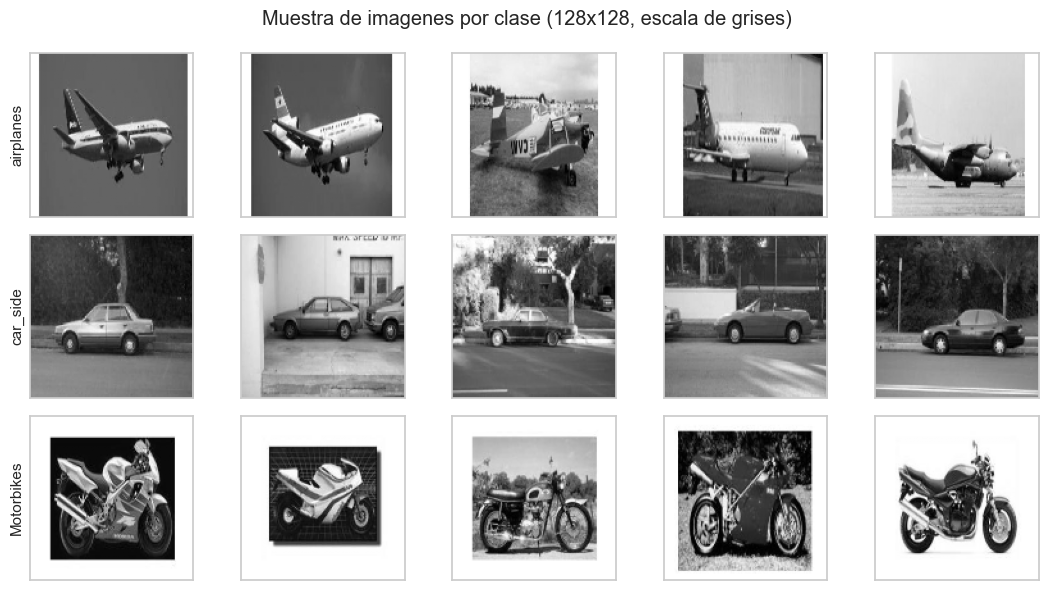
\includegraphics[width=0.85\textwidth]{img/muestras_clase.png}
            \caption{Muestra de imágenes por clase ($128\times128$, escala de grises).}
            \label{fig:muestras}
        \end{figure}

        \item Extraer descriptores SIFT de todas las imágenes.

        Con \texttt{cv2.SIFT\_create()} se aplicó \texttt{detectAndCompute} a cada imagen,
        obteniendo sus \textit{keypoints} y un descriptor de \textbf{128 dimensiones} por
        cada uno. El número de descriptores por imagen es variable: \textbf{mínimo 29,
        máximo 296 y una media de 121}, sin ninguna imagen vacía. La Figura~\ref{fig:sift}
        muestra los \textit{keypoints} detectados sobre una imagen de cada clase; el tamaño
        y la orientación de cada círculo reflejan la escala y la rotación del punto de
        interés.

        \begin{figure}[H]
            \centering
            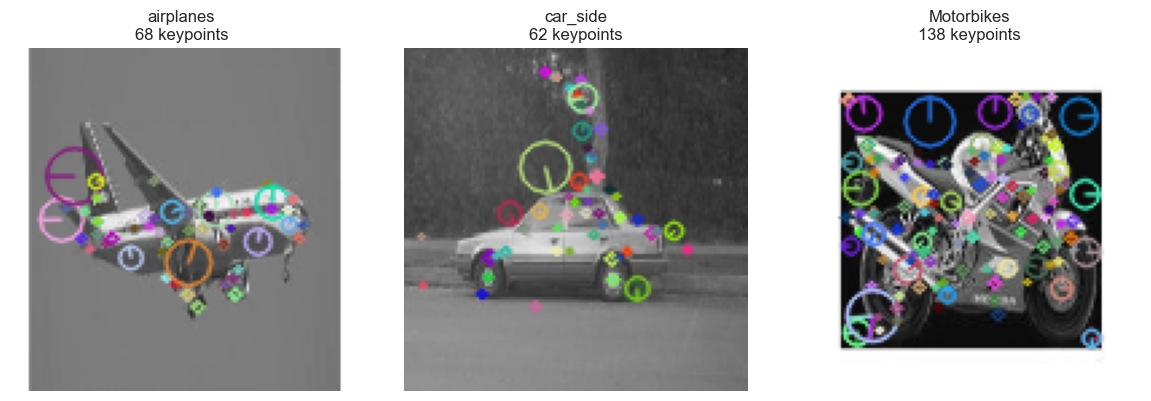
\includegraphics[width=0.95\textwidth]{img/sift_keypoints.png}
            \caption{Keypoints SIFT detectados sobre una imagen representativa de cada clase.}
            \label{fig:sift}
        \end{figure}

        \item Ejecutar k-means con $k$ clusters para obtener el vocabulario.

        Todos los descriptores se apilaron en una única matriz de tamaño
        $43\,612 \times 128$ y se agruparon con \textbf{k-means} ($k = 200$,
        \texttt{n\_init = 3}, quedándose con la mejor de 3 inicializaciones). Cada uno de los
        200 centroides resultantes constituye una \textbf{palabra visual}, de modo que el
        vocabulario visual es una matriz $200 \times 128$. El entrenamiento de k-means tardó
        aproximadamente $6.3$ s.

        \item Para cada imagen, construir su histograma de palabras visuales (Mostrar 5 de cada agrupación).

        Cada descriptor SIFT de una imagen se asigna a la palabra visual más cercana y se
        cuenta su frecuencia, generando un histograma de dimensión $k = 200$
        \textbf{normalizado en L1} (suma 1). La matriz de características resultante tiene
        forma $360 \times 200$. La Figura~\ref{fig:histogramas} muestra cinco histogramas por
        clase: se aprecia que las imágenes de una \textbf{misma clase} producen
        distribuciones de palabras visuales \textbf{parecidas entre sí}, lo que es la base
        del poder discriminativo del modelo.

        \begin{figure}[H]
            \centering
            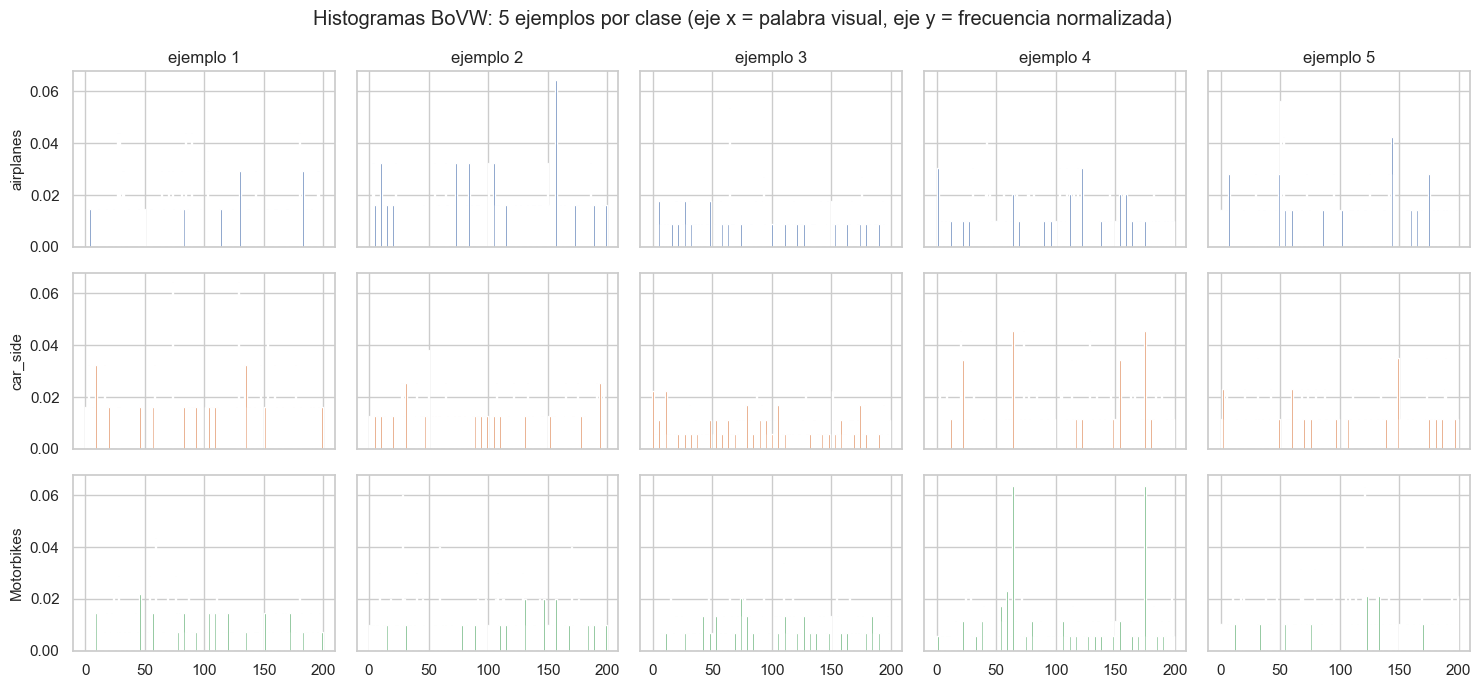
\includegraphics[width=\textwidth]{img/histogramas_bovw.png}
            \caption{Histogramas BoVW: 5 ejemplos por clase (eje $x$ = palabra visual, eje $y$ = frecuencia normalizada).}
            \label{fig:histogramas}
        \end{figure}

        \item Dividir el conjunto en entrenamiento (80\%) y prueba (20\%).

        El conjunto se dividió de forma \textbf{estratificada} (manteniendo la proporción de
        clases) en 80\% de entrenamiento (\textbf{288 imágenes}, 96 por clase) y 20\% de
        prueba (\textbf{72 imágenes}, 24 por clase).

        \item Entrenar un SVM lineal con los histogramas de entrenamiento utilizando búsqueda de hiperparámetros ($grid$ $search$).

        Se entrenó un \textbf{SVM con kernel lineal}, ajustando el parámetro de
        regularización $C$ mediante \textit{grid search} con validación cruzada de 5
        particiones sobre la rejilla $C \in \{0.01, 0.1, 1, 10, 100\}$. El mejor valor
        encontrado fue \textbf{$C = 100$}, con una exactitud media en validación cruzada
        (sobre el conjunto de entrenamiento) de \textbf{$0.8403$}.

        \item Predecir las etiquetas del conjunto de prueba y calcular exactitud, comenta tus resultados.

        Sobre el conjunto de prueba (datos no vistos) el modelo alcanzó una
        \textbf{exactitud de $0.8472$ ($\approx 85\%$)}. El reporte de clasificación por
        clase se muestra en la Tabla~\ref{tab:reporte}.

        \begin{table}[H]
            \centering
            \begin{tabular}{lccc}
                \toprule
                Clase & Precisión & Recall & F1-score \\
                \midrule
                airplanes  & 0.84 & 0.88 & 0.86 \\
                car\_side  & 0.79 & 0.96 & 0.87 \\
                Motorbikes & 0.94 & 0.71 & 0.81 \\
                \midrule
                \textbf{Exactitud global} & \multicolumn{3}{c}{\textbf{0.85} (72 imágenes)} \\
                \bottomrule
            \end{tabular}
            \caption{Métricas por clase del SVM lineal ($k = 200$) sobre el conjunto de prueba.}
            \label{tab:reporte}
        \end{table}

        \textbf{Comentario:} El modelo BoVW + SVM lineal alcanza una exactitud cercana al
        85\%, muy por encima del azar ($33\%$ para 3 clases balanceadas). La clase
        \texttt{car\_side} es la que mejor se recupera (\textit{recall} de 0.96), mientras
        que \texttt{Motorbikes} presenta una precisión muy alta (0.94) pero un
        \textit{recall} más bajo (0.71): el clasificador rara vez confunde otra clase con una
        moto, pero sí deja escapar algunas motos hacia las otras categorías.

        \item Mostrar la matriz de confusión, comenta tus resultados.

        La Figura~\ref{fig:confusion} muestra la matriz de confusión. La diagonal concentra
        la gran mayoría de las predicciones, lo que confirma la buena separación de las
        clases. Los pocos errores se reparten principalmente entre \texttt{airplanes} y
        \texttt{Motorbikes}, clases que comparten estructuras locales similares (bordes
        alargados, fondos uniformes), mientras que \texttt{car\_side} resulta la categoría
        más fácilmente separable.

        \begin{figure}[H]
            \centering
            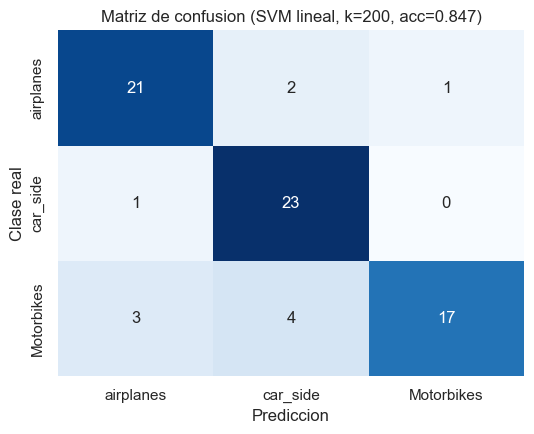
\includegraphics[width=0.6\textwidth]{img/matriz_confusion.png}
            \caption{Matriz de confusión del SVM lineal ($k = 200$, exactitud $= 0.847$).}
            \label{fig:confusion}
        \end{figure}
    \end{enumerate}


\item \textbf{Evaluación y comparación de resultados: }
    \begin{enumerate}
        \item \textbf{Variar el número de palabras visuales} ($k = 50, 200, 500$). ¿Cómo afecta la exactitud y el tiempo de cómputo?

        Reutilizando la misma partición de entrenamiento/prueba para una comparación justa,
        se repitió todo el proceso con tres tamaños de vocabulario. Los resultados se resumen
        en la Tabla~\ref{tab:k} y la Figura~\ref{fig:k}.

        \begin{table}[H]
            \centering
            \begin{tabular}{ccccc}
                \toprule
                $k$ & Exactitud & Mejor $C$ & $t_{\text{k-means}}$ & $t_{\text{total}}$ \\
                \midrule
                50  & 0.7500 & 10  & 2.2 s  & 2.3 s  \\
                200 & 0.8472 & 100 & 5.9 s  & 6.0 s  \\
                500 & 0.8333 & 100 & 12.6 s & 12.7 s \\
                \bottomrule
            \end{tabular}
            \caption{Exactitud y tiempo de cómputo en función del tamaño del vocabulario $k$.}
            \label{tab:k}
        \end{table}

        \begin{figure}[H]
            \centering
            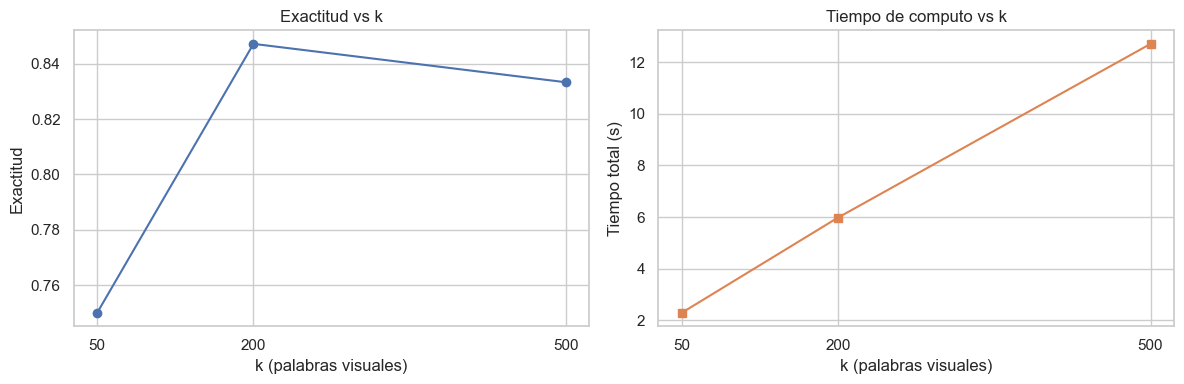
\includegraphics[width=\textwidth]{img/exactitud_vs_k.png}
            \caption{Exactitud (izquierda) y tiempo total de cómputo (derecha) frente a $k$.}
            \label{fig:k}
        \end{figure}

        \textbf{Comentario:} Al aumentar $k$ el vocabulario es más expresivo y la exactitud
        crece de forma notable de $k=50$ ($0.75$) a $k=200$ ($0.85$); sin embargo, al pasar a
        $k=500$ la exactitud \textbf{deja de mejorar e incluso baja ligeramente} ($0.83$),
        señal de que los histogramas se vuelven muy dispersos y empieza a aparecer
        sobreajuste. El \textbf{tiempo de cómputo}, en cambio, crece de manera marcada (sobre
        todo el de k-means, que casi se duplica en cada salto). El valor $k \approx 200$
        ofrece el mejor compromiso entre exactitud y costo.

        \item \textbf{Cambiar el clasificador}: sustituir SVM por Random Forest  y comparar resultados.

        Con el mismo vocabulario ($k = 200$) se entrenó un \textbf{Random Forest} ajustando
        por \textit{grid search} el número de árboles y la profundidad máxima
        (\texttt{n\_estimators} $\in \{100, 300\}$, \texttt{max\_depth} $\in \{$None$, 20\}$).
        Los mejores parámetros fueron \texttt{n\_estimators = 300} y
        \texttt{max\_depth = None}. La comparación se resume en la Tabla~\ref{tab:clf} y la
        Figura~\ref{fig:clf}.

        \begin{table}[H]
            \centering
            \begin{tabular}{lc}
                \toprule
                Clasificador & Exactitud (prueba) \\
                \midrule
                SVM lineal    & 0.8472 \\
                Random Forest & 0.8333 \\
                \bottomrule
            \end{tabular}
            \caption{Comparación de clasificadores con $k = 200$.}
            \label{tab:clf}
        \end{table}

        \begin{figure}[H]
            \centering
            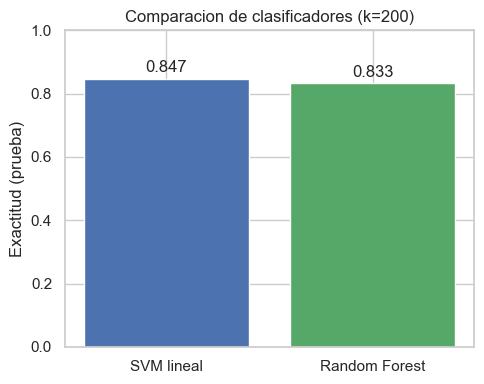
\includegraphics[width=0.5\textwidth]{img/comparacion_clasificadores.png}
            \caption{Comparación de exactitud entre SVM lineal y Random Forest ($k = 200$).}
            \label{fig:clf}
        \end{figure}

        \textbf{Comentario:} Con el mismo vocabulario, el SVM lineal ($0.847$) y el Random
        Forest ($0.833$) ofrecen resultados \textbf{muy comparables}; la diferencia es de
        apenas una imagen. El SVM lineal resulta ligeramente superior y más económico de
        entrenar, lo cual es coherente con que los histogramas normalizados son
        representaciones de dimensión moderada sobre las que un separador lineal funciona muy
        bien.

        \item \textbf{Agregar validación cruzada}: hacer validación cruzada con 5 particiones e informar la media y desviación estándar de la exactitud.

        Para obtener una estimación más fiable que la de una única partición 80/20, se
        realizó \textbf{validación cruzada estratificada de 5 particiones} sobre todo el
        conjunto, empleando los mejores hiperparámetros hallados para cada modelo. Los
        resultados se muestran en la Tabla~\ref{tab:cv} y la Figura~\ref{fig:cv}.

        \begin{table}[H]
            \centering
            \begin{tabular}{lcc}
                \toprule
                Clasificador & Media & Desviación estándar \\
                \midrule
                SVM lineal    & 0.8722 & 0.0297 \\
                Random Forest & 0.8833 & 0.0286 \\
                \bottomrule
            \end{tabular}
            \caption{Exactitud en validación cruzada de 5 particiones.}
            \label{tab:cv}
        \end{table}

        \begin{figure}[H]
            \centering
            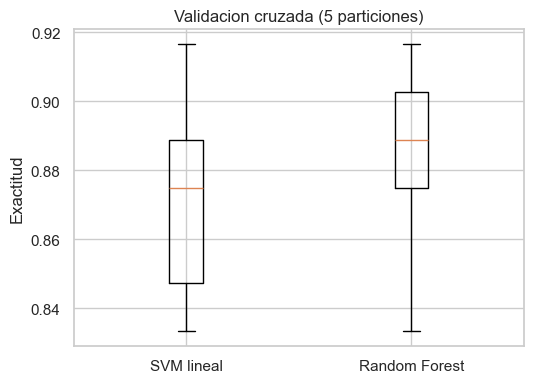
\includegraphics[width=0.55\textwidth]{img/validacion_cruzada.png}
            \caption{Distribución de la exactitud en las 5 particiones (boxplot).}
            \label{fig:cv}
        \end{figure}

        \textbf{Comentario:} Con 5 particiones la exactitud media se sitúa en torno a
        $0.87$--$0.88$ para ambos clasificadores, con una \textbf{desviación estándar
        pequeña} ($\approx 0.03$), lo que indica que el modelo es \textbf{estable} y que el
        resultado de la partición única (inciso~g) no fue fortuito. Ambos clasificadores son
        estadísticamente equivalentes: sus intervalos se solapan ampliamente.

    \end{enumerate}

\item \textbf{Opcional}
    \begin{enumerate}
        \item \textbf{Utilizar una base de datos diferente}y repetir la implementación del modelo adaptando la carga de datos.
    \end{enumerate}

\item \textbf{Preguntas:}

    \begin{itemize}
        \item ¿Por qué es necesario normalizar los histogramas?

        Porque cada imagen genera un número distinto de descriptores SIFT (depende de su
        tamaño, textura y cantidad de \textit{keypoints} detectados). Si no se normaliza, una
        imagen con muchos \textit{keypoints} tendría conteos absolutos mayores y el
        clasificador compararía \textit{magnitudes} en lugar de la \textit{distribución} de
        palabras visuales. Al normalizar (L1, que el histograma sume 1) el vector representa
        \textbf{proporciones} de cada palabra visual, lo que lo hace invariante al número
        total de descriptores y pone todas las imágenes en una escala comparable; esto además
        favorece el buen comportamiento del SVM lineal.

        \item ¿Qué ocurre si $k$ es demasiado pequeño? ¿y si es demasiado grande?

        Con $k$ \textbf{demasiado pequeño}, las palabras visuales son muy genéricas:
        estructuras locales distintas caen en la misma palabra, los histogramas pierden poder
        discriminativo y el modelo \textbf{subajusta} (las clases se confunden). Con $k$
        \textbf{demasiado grande}, las palabras son muy específicas: los histogramas se
        vuelven muy dispersos (\textit{sparse}), aparece riesgo de \textbf{sobreajuste}, se
        necesita más cantidad de datos y crece mucho el costo de k-means y de la asignación;
        la exactitud se estanca o incluso baja (como se observa en el inciso 2(a)). Existe un
        valor intermedio óptimo ($\approx 200$ en este caso).

        \item ¿Podría utilizarse este método para detección de objetos en lugar de clasificación?

        Sí, pero no directamente. La clasificación BoVW describe \textbf{toda la imagen} con
        un único histograma y por tanto \textbf{no localiza} el objeto. Para detección habría
        que aplicar BoVW sobre \textbf{regiones candidatas} (ventanas deslizantes /
        \textit{sliding window} o \textit{region proposals}) y clasificar cada región, o
        incorporar información espacial (p.\,ej.\ \textit{spatial pyramids}). Es decir, BoVW
        sirve como \textbf{descriptor de región} dentro de un esquema de detección, no como
        detector por sí solo.
    \end{itemize}

\end{enumerate}

\bigskip


\section{Código}
El código fuente completo de la práctica se encuentra implementado en el cuaderno de Jupyter
\texttt{Practica\_5\_Agrupamiento\_y\_Clasificacion.ipynb}, que \textbf{se adjunta junto con
este reporte}. En dicho cuaderno se documenta, celda por celda, todo el flujo descrito en la
sección de Desarrollo (carga y filtrado del dataset, extracción de descriptores SIFT,
construcción del vocabulario con k-means, generación de los histogramas, entrenamiento del
SVM y del Random Forest, y las evaluaciones comparativas).

\section{Conclusiones}
Se implementó por completo el modelo de \textbf{Bolsa de Palabras Visuales (BoVW)} para
clasificar imágenes de 3 categorías de Caltech-101 (\texttt{airplanes}, \texttt{car\_side},
\texttt{Motorbikes}). El flujo SIFT $\rightarrow$ k-means (vocabulario visual)
$\rightarrow$ histograma normalizado $\rightarrow$ clasificador reproduce fielmente lo visto
en clase y alcanza una exactitud de $\approx 85\%$ en prueba y $\approx 0.87$ en validación
cruzada de 5 particiones, muy por encima del azar ($33\%$).

Principales conclusiones:

\begin{itemize}
    \item El \textbf{tamaño del vocabulario $k$} es el hiperparámetro más influyente: la
    exactitud crece con rendimientos decrecientes y el tiempo de cómputo aumenta de forma
    marcada; $k \approx 200$ fue el mejor compromiso.
    \item La \textbf{normalización de los histogramas} es esencial para que la
    representación sea invariante al número de descriptores.
    \item \textbf{SVM lineal} y \textbf{Random Forest} dan resultados comparables; la
    validación cruzada confirma que el modelo es estable (baja desviación estándar).
    \item Los errores se concentran entre clases que comparten apariencia local
    (\texttt{airplanes} vs \texttt{Motorbikes}), mientras que \texttt{car\_side} se separa
    con facilidad.
    \item El pipeline es \textbf{genérico y reutilizable}: aplicarlo a otra base de datos
    solo exige cambiar la carga de datos.
\end{itemize}

\section{Referencias}

    \begin{itemize}
    \item D. G. Lowe, "Distinctive image features from scale-invariant keypoints", IJCV 2004.
    \item G. Csurka et al., "Visual categorization with bags of keypoints", ECCV 2004.
    \item Scikit-learn documentation: \url{https://scikit-learn.org}
    \item OpenCV Python tutorials: \url{https://docs.opencv.org}


    \end{itemize}

% \end{enumerate}   % <- cierre sobrante del documento original; se neutraliza para que el reporte compile (no se elimina contenido).


\end{document}
